\documentclass[a4paper, 12pt]{article}

\usepackage[utf8]{inputenc}
\usepackage[spanish]{babel}
\usepackage[margin=2cm]{geometry}
\usepackage{graphicx}
\usepackage{float}
\usepackage{pdfpages}

\title{		\textbf{Trabajo Práctico 1}\\
			\textbf{Conjunto de instrucciones MIPS}
			}

\author{	Lucas Medrano, \textit{Padrón Nro. 00.000}                     \\
            \texttt{ dirección de e-mail }                                              \\
            Federico Álvarez, \textit{Padrón Nro. 00.000}                     \\
            \texttt{ dirección de e-mail }                                              \\
            Facundo Fernández, \textit{Padrón Nro. 89.843}                     \\
            \texttt{ ffelfis@gmail.com}                                              \\[2.5ex]
            \normalsize{Grupo Nro. \quad - 2do. Cuatrimestre de 2018}                       \\
            \normalsize{66.20 Organización de Computadoras}                             \\
            \normalsize{Facultad de Ingeniería, Universidad de Buenos Aires}            \\
       }
\date{}

\begin{document}
	\maketitle
	\thispagestyle{empty}
	\begin{abstract}
		Este artículo es un modelo que proporciona a los alumnos las instrucciones necesarias para preparar sus informes para la asignatura \textit{66.20 Organización de Computadoras}. El informe deberá contener un resumen de no más de 150 palabras. La primera página del artículo deberá seguir el formato que se ilustra en el presente modelo y deberá contener el título, los nombres de los autores, sus números de padrón, sus direcciones de e-mail, número de grupo y el resumen. La primera página del informe no debe ser numerada.
	\end{abstract}
	
	\pagebreak
	\thispagestyle{empty}
	\tableofcontents
	\newpage
	\setcounter{page}{1}
	\section{Enunciado}
	\begin{figure}[H]
		\centering
		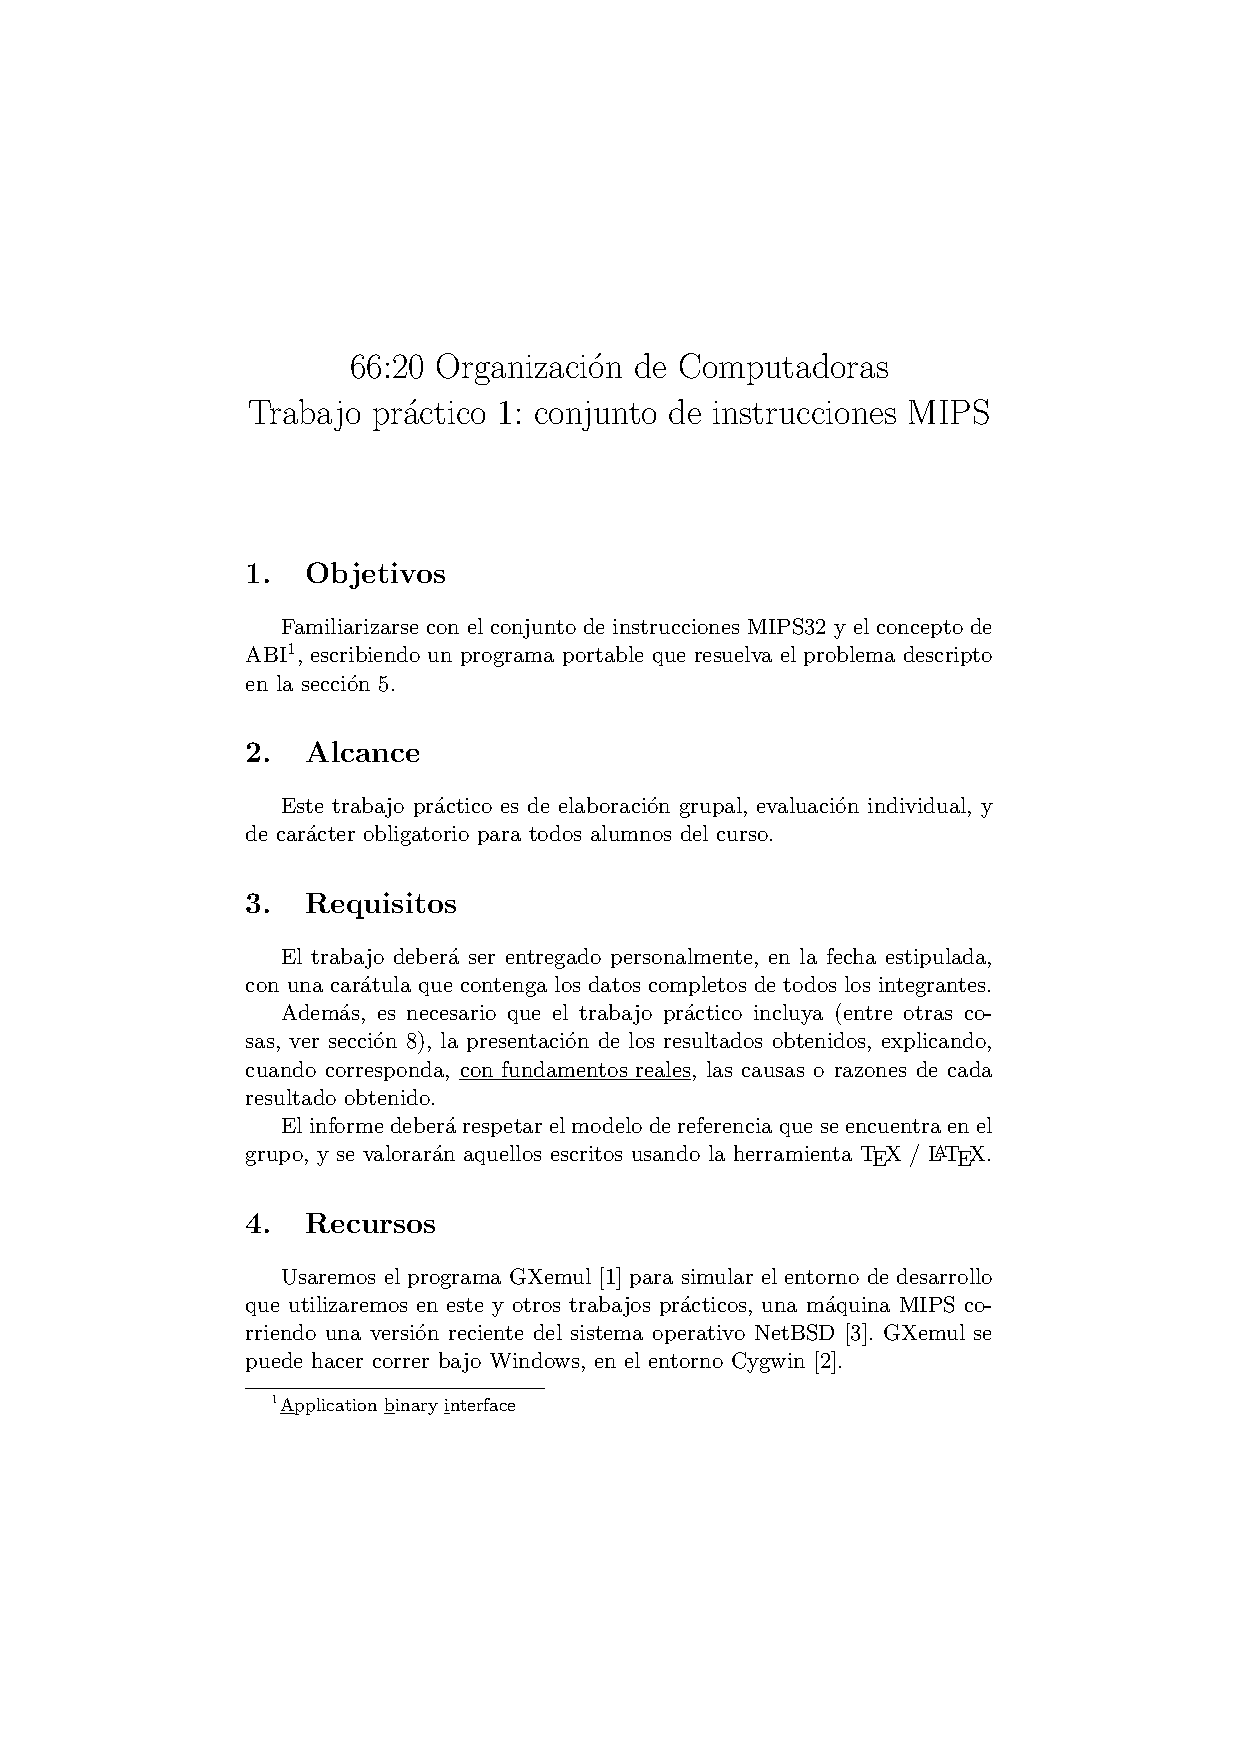
\includegraphics[scale=1, page = 1, clip, trim=20mm 36mm 20mm 35mm]{files/enunciado.pdf}
	\end{figure}
	
	\newpage
	\begin{figure}[H]
		\centering
		\includegraphics[scale=1, page = 2, clip, trim=20mm 36mm 20mm 20mm]{files/enunciado.pdf}
	\end{figure}
	
	\newpage
	\begin{figure}[H]
		\centering
		\includegraphics[scale=1, page = 3, clip, trim=20mm 36mm 20mm 20mm]{files/enunciado.pdf}
	\end{figure}
	
	\newpage
	\begin{figure}[H]
		\centering
		\includegraphics[scale=1, page = 4, clip, trim=20mm 36mm 20mm 20mm]{files/enunciado.pdf}
	\end{figure}
	
	\newpage
	\begin{figure}[H]
		\centering
		\includegraphics[scale=1, page = 5, clip, trim=20mm 36mm 20mm 20mm]{files/enunciado.pdf}
	\end{figure}
	
	
	
	%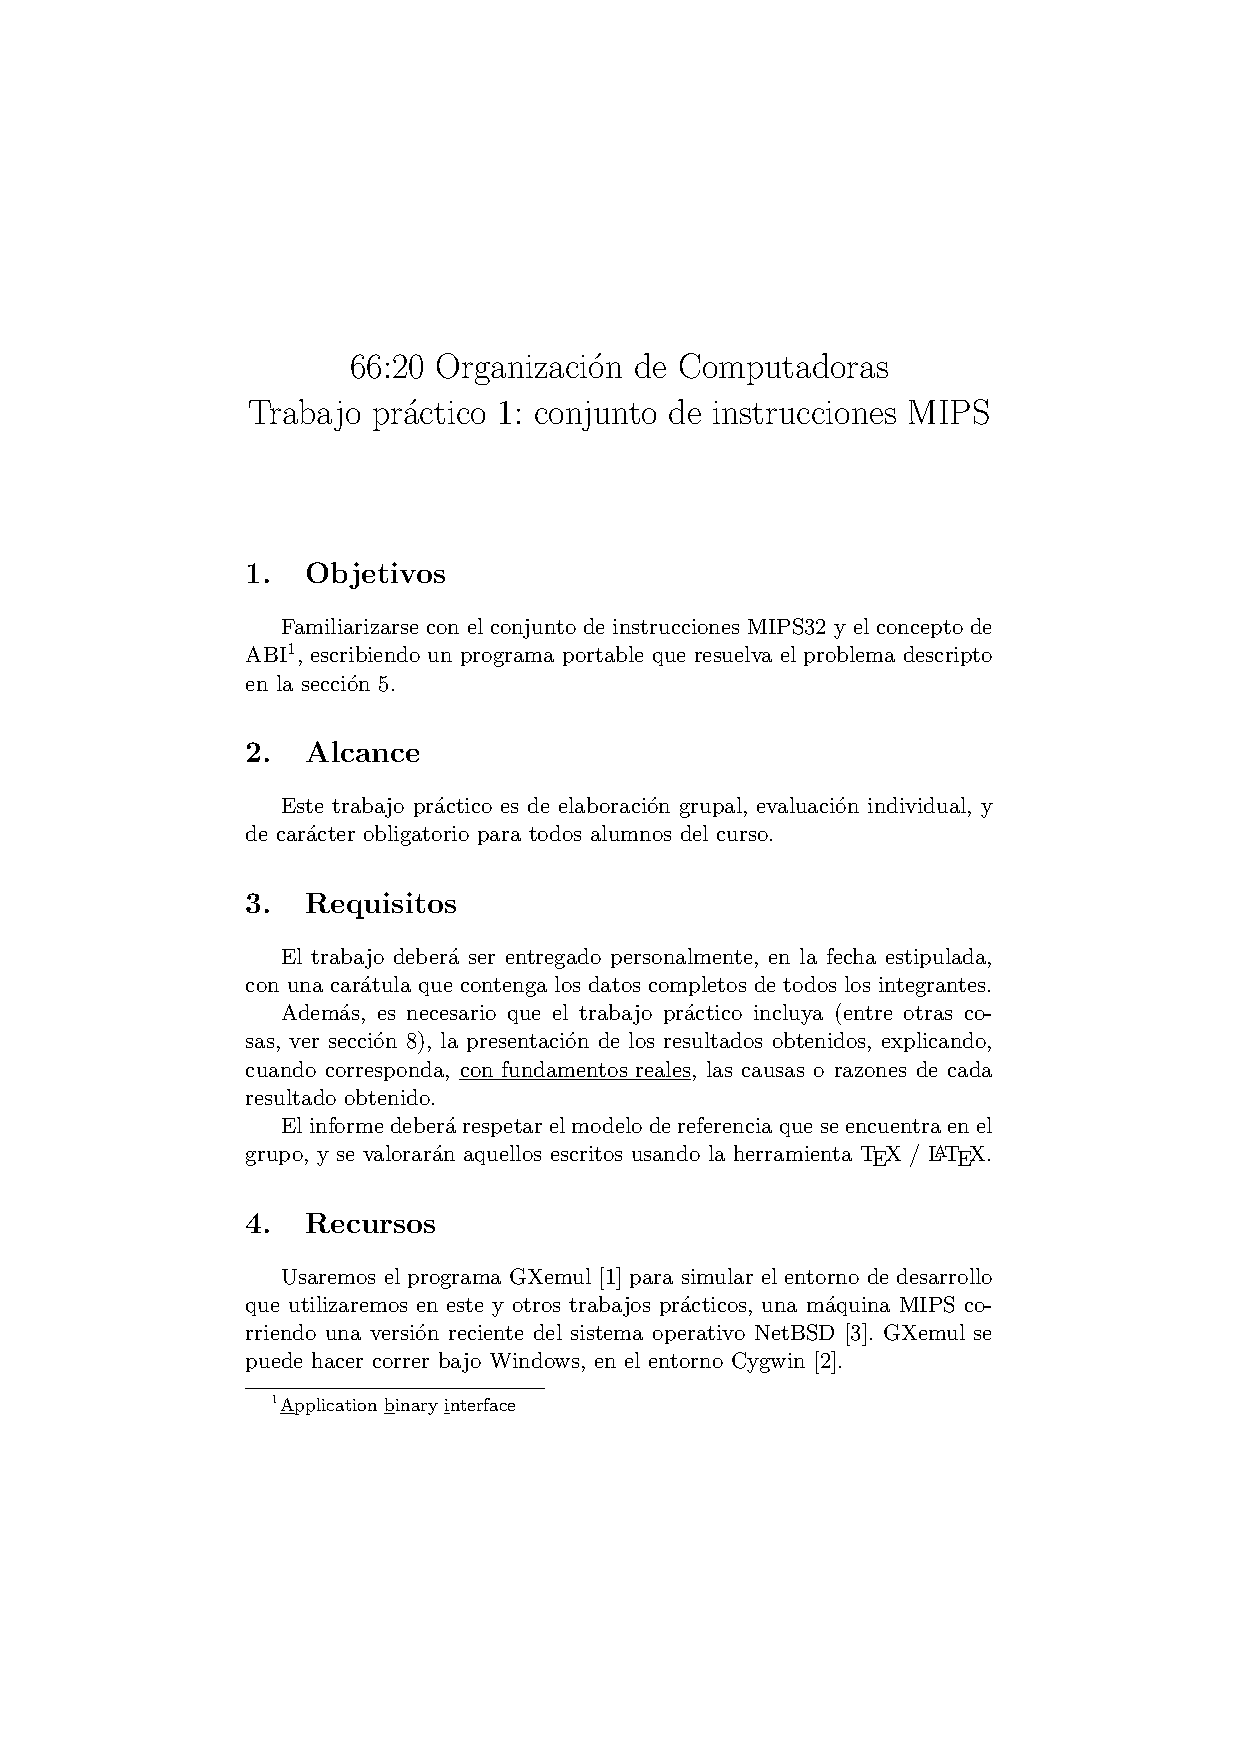
\includepdf[scale=1, pages=1-1]{files/enunciado.pdf} 
	%clip, trim=0mm 36mm 0mm 0mm, offset=0 36

	\section{Implementación}
	
	\section{Pruebas}
	
	\section{Diagramas de stack}
	
	\section{Código fuente}
\end{document}
